\documentclass[]{report}

\usepackage{graphicx}
\usepackage{float}
\usepackage{amsmath}
\usepackage{amsfonts}
\usepackage{wasysym}
\usepackage{listings}
\usepackage{xcolor}
\lstset{
	basicstyle=\ttfamily,
	columns=fullflexible,
	frame=L,
	showstringspaces=false, 
	commentstyle=\color{green},
	breaklines=true,
	postbreak=\mbox{\textcolor{red}{$\hookrightarrow$}\space},
}
\pagenumbering{Roman}
% Title Page
\title{MCEN 3047 - Homework 3}
\author{Jack Reilly Goldrick}


\begin{document}
	\maketitle
	
\section{Problem 1}

\subsection{Part A \& B}
\begin{itemize}


\item Mean: 
	\subitem{Indoor: }    9.842105
	\subitem{Outdoor: }     7.773684

\item Std: 
	\subitem{Indoor: }     1.844305
	\subitem{Outdoor: }     0.983103

\item Median: 	
	\subitem{Indoor: }   9.4
	\subitem{Outdoor: }  7.6

\item Mode: 
	\subitem{Indoor: }  9.2
	\subitem{Outdoor: } 7.2

	
\end{itemize}

\subsection{Part C}

\begin{figure}[H]
	\centering
	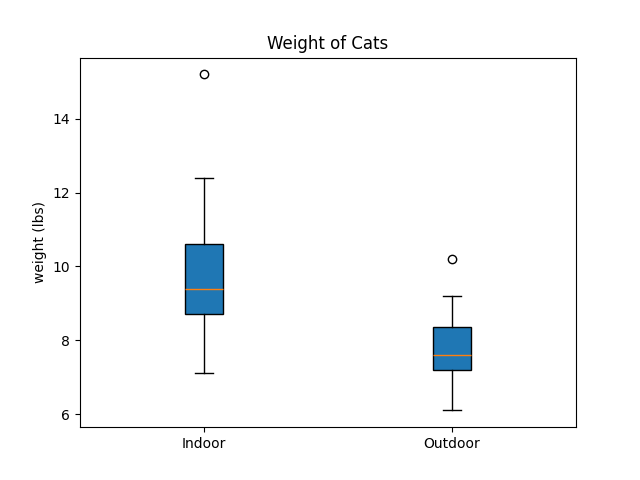
\includegraphics[width=0.7\linewidth]{pics/1.c}
	\caption{Box Plot where Each Category has 1 outlier defined by the Open Circle}
	\label{fig:1}
\end{figure}


\subsection{Part D}

\begin{figure}[H]
	\centering
	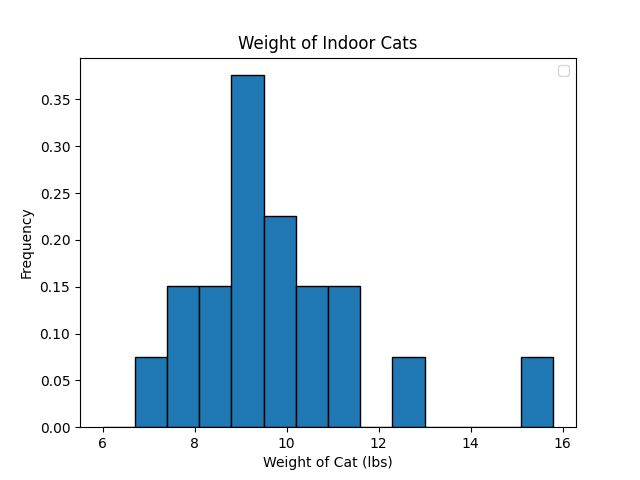
\includegraphics[width=0.7\linewidth]{pics/1.d.in}
	\caption{Indoor Histogram}
	\label{fig:2}
\end{figure}

\begin{figure}[H]
	\centering
	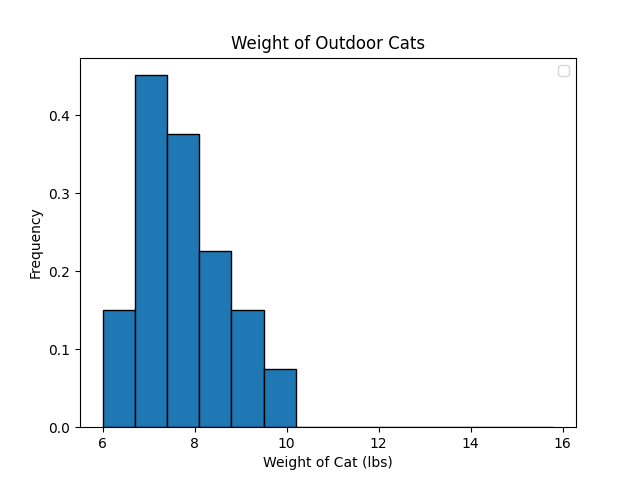
\includegraphics[width=0.7\linewidth]{pics/1.d.out}
	\caption{Outdoor Histogram}
	\label{fig:3}
\end{figure}

\subsection{Part E}

\begin{figure}[H]
	\centering
	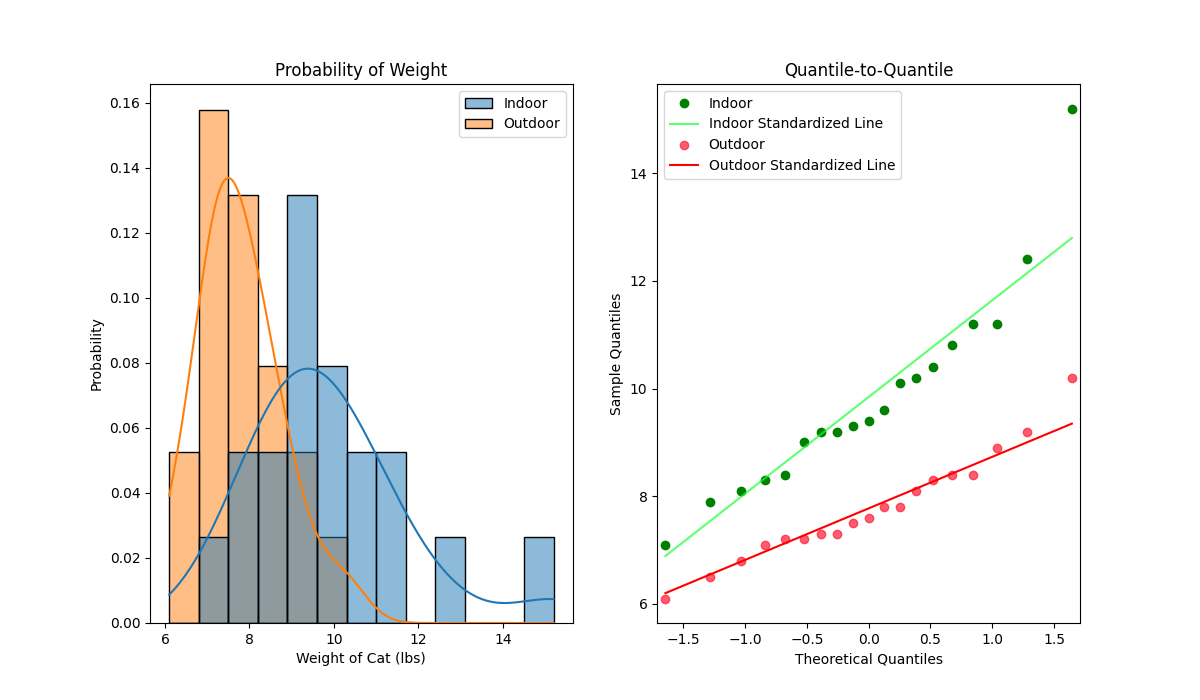
\includegraphics[width=1\linewidth]{pics/1.e}
	\caption{Norm Plot with a QQ-Plot that clearly shows the distribution models the data well}
	\label{fig:4}
\end{figure}

\subsection{Part F}


\begin{figure}[H]
	\centering
	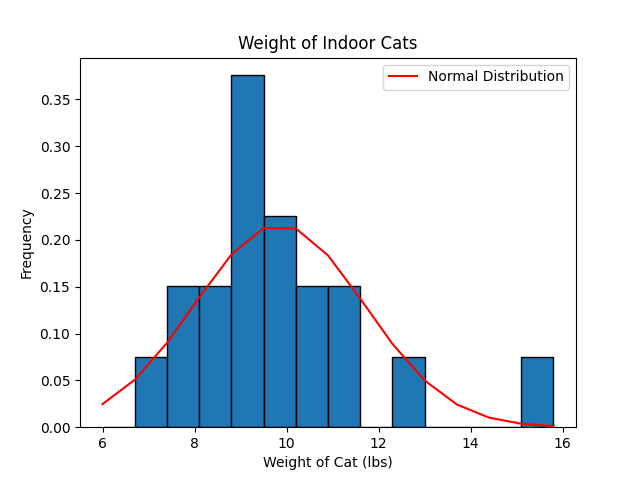
\includegraphics[width=1\linewidth]{pics/1.f.in}
	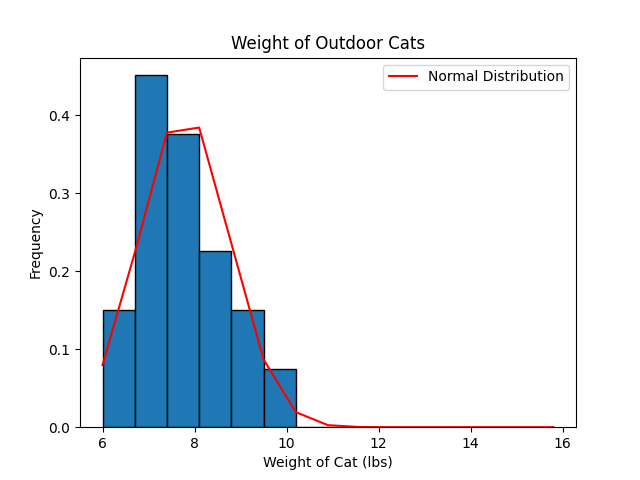
\includegraphics[width=1\linewidth]{pics/1.f.out}
	\caption{The Figure Shows the Distribution is an accurate Representation of the Data due to the high similarity}
	\label{fig:5}
\end{figure}

\section{Problem 2}

\subsection{Part A}

\begin{itemize}
	\item Let $I = [0, 120] \subset \mathbb{R}$
	
	\item Let $(I, \ \mathcal{P}(I), \ \mu) $ be a Probability Space such that:
	
	\begin{itemize}
		\item $\mu(I) = 1$
		
		\item $ \mathbf{X} : \mathcal{P}(I) \rightarrow \mathbb{R} $ is an Independent Variable with
		
			\begin{itemize}
				\item $f_{x}: \mathbb{R} \rightarrow [0, \infty]$ such that
			\end{itemize}
			
			$$ f_{x} = \frac{x - 20}{5000} $$
		
		\item Thus by definition, Since the measure sends a variable to the interval $[0, 1]$  we have:
		
		\begin{itemize}
			\item $\mu(\mathcal{P}(I)) = P_{x} (\mathcal{P}(I) ) =  \int_{\mathcal{P}(I)}  f_{x}(x) \, dx$
		\end{itemize}
	\end{itemize}
	
	\item Thus the portion of students who take (60, 120) minutes is defined as:
	
	\begin{itemize}
	\item $P_{x} ([60, 120] ) = \int_{[60, 120]}  f_{x}(x) \, dx =  \int_{60}^{120} \frac{x - 20}{5000} \, dx$
	
	
		\begin{itemize}
			\item Therefore the portion is $84 \% $ of the students
		\end{itemize}
	\end{itemize}
\end{itemize}
	
	\subsection{Part B}
	
		\begin{itemize}
			\item Measuring the Expected Value of the Independent Variable $X$, $\mathbf{EX}$, with  $f_{x}: \mathbb{R} \rightarrow [0, \infty]$ we have:
			
			$$ \mathbf{EX} = \int_{I} x f_{x}(x) \, dx =  \int_{20}^{120} \frac{x^2 - 20x}{5000} \, dx $$
			
			$$ \mathbf{EX} = 86 \ \frac{2}{3}  \ \text{Minutes} $$
			
			
		\end{itemize}
	
	\subsection{Part C}
	
		\begin{itemize}
			\item Measuring the Standard Deviation of the Independent Variable $X$, $\sigma$, with  $f_{x}: \mathbb{R} \rightarrow [0, \infty]$ we have:
			
			$$ \sigma = \left( \int_{I} (x - \mathbf{EX})^2  f_{x}(x) \, dx \right)^{\frac{1}{2}} =  \left(\int_{20}^{120} (x - \frac{260}{3}) \frac{x- 20}{5000} \, dx \right)^{\frac{1}{2}}  $$
			
			$$ \sigma = 23.570 \ \text{Minutes} $$
			
			
		\end{itemize}
		
		
		
\section{Problem 3}


	\subsection{Part A}
	
	\begin{itemize}
		\item Let $I = [0, \infty] \subset \mathbb{R}$
		
		\item Let $(I, \ \mathcal{P}(I), \ \mu) $ be a Probability Space such that:
		
		\begin{itemize}
			\item $\mu(I) = 1$
			
			\item $ \mathbf{X} : \mathcal{P}(I) \rightarrow \mathbb{R} $ is an Independent Variable with
			
			\begin{itemize}
				\item $f_{x}: \mathbb{R} \rightarrow [0, \infty]$ such that
			\end{itemize}
			
			$$ f_{x} = \frac1{\sqrt{2\pi\sigma^2}}{e}^{- \frac{1}{2} (\frac{x-\mu}{\sigma})^2}$$
			
			\item Thus by definition, Since the measure sends a variable to the interval $[0, 1]$  we have:
			
			\begin{itemize}
				\item $\mu(\mathcal{P}(I)) = P_{x} (\mathcal{P}(I) ) =  \int_{\mathcal{P}(I)}  f_{x}(x) \, dx$
			\end{itemize}
		\end{itemize}
		
		\item Thus the Probability of  $\mathcal{P}(I)  = \{[24000, \infty]\}$ is defined as:
		
		\begin{itemize}
			\item $P_{x} ([24000, \infty] ) = \int_{[24000, \infty]}  f_{x}(x) \, dx =  \int_{24000}^{\infty}  \frac1{\sqrt{2\pi\sigma^2}}{e}^{- \frac{1}{2} (\frac{x-\mu}{\sigma})^2} \, dx$
			
			
			\begin{itemize}
				\item Therefore the probability a light lasts more than 24000 hrs is 
				
				$$74.7507 \%$$
			\end{itemize}
		\end{itemize}
	\end{itemize}
	
	\subsection{Part B}
	
		\begin{itemize}
			\item Using The Cumaltive Distribution Function we have:
			
				$P_{x} (\mathbf{X} \leq 26012 ) = \int_{[0, 26012] }  f_{x}(x) \, dx =  \int_{0}^{26012}  \frac1{\sqrt{2\pi\sigma^2}}{e}^{- \frac{1}{2} (\frac{x-\mu}{\sigma})^2} \, dx$
				
		\end{itemize}

		$$ P_{x} (\mathbf{X} \leq 26012 ) \approx 75.00\% $$
		
		
	\subsection{Part C}
	
		\begin{itemize}
			\item Using The Cumaltive Distribution Function we have:
			
			$P_{x} (\mathbf{X} \leq 27500 ) = \int_{[0, 27500] }  f_{x}(x) \, dx =  \int_{0}^{27500}  \frac1{\sqrt{2\pi\sigma^2}}{e}^{- \frac{1}{2} (\frac{x-\mu}{\sigma})^2} \, dx$
			
		\end{itemize}
		
		$$ P_{x} (\mathbf{X} \leq 27500 ) \approx 95.22 \ \text{Percentile}$$



	\subsection{Part D}
	
	
		\begin{itemize}
			\item Using The Measure of the Probability Density Function we have:
			
			$P_{x} (20000 < \mathbf{X} < 30000 ) = \int_{[20000, 30000] }  f_{x}(x) \, dx =  \int_{20000}^{30000}  \frac1{\sqrt{2\pi\sigma^2}}{e}^{- \frac{1}{2} (\frac{x-\mu}{\sigma})^2} \, dx$
			
		\end{itemize}
		
		$$ P_{x} (20000 < \mathbf{X} < 30000 ) \approx 99.22 \ \text{Percentile}$$




	\section{Problem 4}
	
	
	
		\subsection{Part A}
		
		\begin{itemize}
			\item Mean: 86.67018074199994
			
			\item Variance:  555.912639
			
			
			
		\end{itemize}
		
		\subsection{Part B}
			
			\begin{figure}[H]
				\centering
				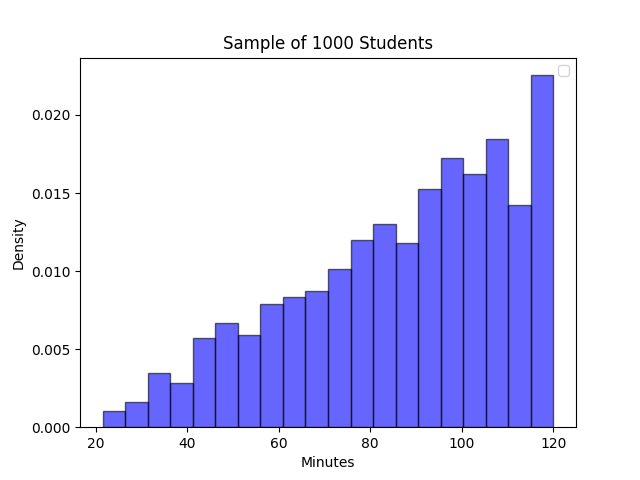
\includegraphics[width=1\linewidth]{pics/4.b}
				\caption{}
				\label{fig:6}
			\end{figure}
			
		
		
		\subsection{Part C}
		
			
			\begin{figure}[H]
				\centering
				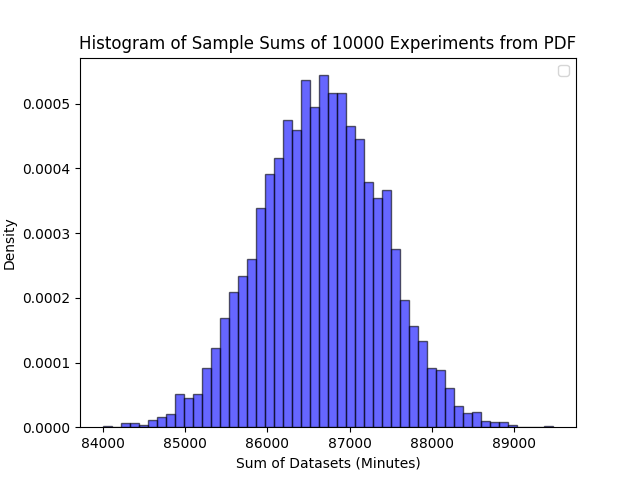
\includegraphics[width=1\linewidth]{pics/4.c}
				\caption{}
				\label{fig:7}
			\end{figure}
		
		
		
		\subsection{Part D}
		
		
		\begin{figure}[H]
			\centering
			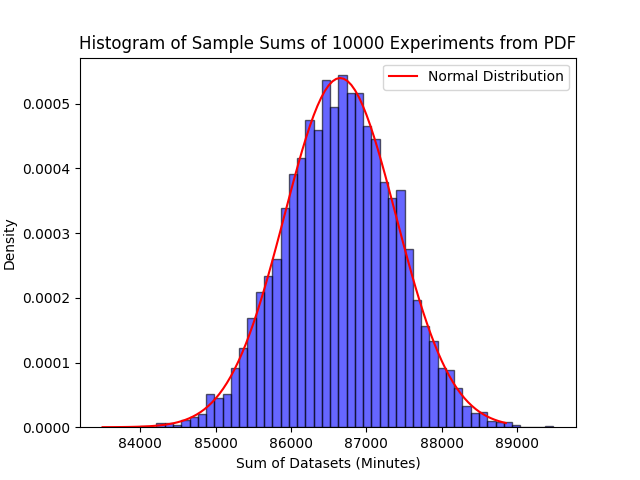
\includegraphics[width=1\linewidth]{pics/4.d}
			\caption{}
			\label{fig:8}
		\end{figure}
		
		
		\begin{itemize}
			\item       Mean: 86670.180742
			\item		Variance: 558185.236937
			
			\item Both the Mean and Variance are approximately scaled proportionally by the number of summed samples.
		\end{itemize}
		
			\newpage
		
		\section{Code}
		
		
		\lstinputlisting[language=python]{../src/set_4.py}
		
\end{document}